% tikzpic.tex
\documentclass[crop,tikz]{standalone}% 'crop' is the default for v1.0, before it was 'preview'

\usetikzlibrary{arrows,decorations.pathmorphing,decorations.pathreplacing,backgrounds,positioning,fit,matrix}
\usetikzlibrary{shapes,calc,patterns,arrows.meta}
\tikzset{
	vert/.style={circle,inner sep=1.5,fill=white,draw,minimum size=.3cm},
	edge/.style={color=black, thick},
	diredge/.style={->,>={Stealth[width=8pt,length=8pt]},color=black, thick},
	timelabel/.style={fill=white,font=\footnotesize, text centered},
	wave/.style={decorate,decoration={coil,aspect=0}},
	dirwave/.style={->, >={Stealth[width=8pt,length=8pt]},decorate,decoration={coil,aspect=0}},
	diredge2/.style={->,>={Stealth[width=8pt,length=8pt]}}
}
\begin{document}
	
	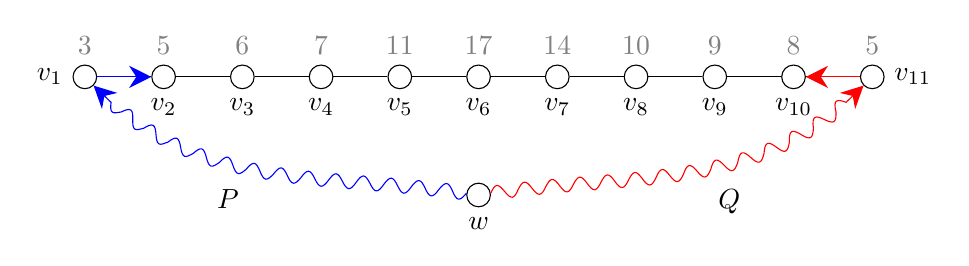
\begin{tikzpicture}
		%%%S_uv
		\node[vert,label=left:$v_1$,label={[text=gray]above:$3$}] (v1) at (1,0) {};
		\node[vert,label=below:$v_2$,label={[text=gray]above:$5$}] (v2) at (2,0) {};
		\node[vert,label=below:$v_3$,label={[text=gray]above:$6$}] (v3) at (3,0) {};
		\node[vert,label=below:$v_4$,label={[text=gray]above:$7$}] (v4) at (4,0) {};
		\node[vert,label=below:$v_5$,label={[text=gray]above:$11$}] (v5) at (5,0) {};
		\node[vert,label=below:$v_6$,label={[text=gray]above:$17$}] (v6) at (6,0) {};
		\node[vert,label=below:$v_7$,label={[text=gray]above:$14$}] (v7) at (7,0) {};
		\node[vert,label=below:$v_8$,label={[text=gray]above:$10$}] (v8) at (8,0) {};
		\node[vert,label=below:$v_9$,label={[text=gray]above:$9$}] (v9) at (9,0) {};
		\node[vert,label=below:$v_{10}$,label={[text=gray]above:$8$}] (v10) at (10,0) {};
		\node[vert,label=right:$v_{11}$,label={[text=gray]above:$5$}] (v11) at (11,0) {};
		\draw (v1) -- (v2) -- (v3) -- (v4) -- (v5) -- 
		(v6) -- (v7) -- (v8) -- 
		(v9) -- (v10) --  (v11);
		
		%%%% node w
		\node[vert,label=below:$w$] (w) at (6,-1.5) {};
		
		
		
		\draw [blue] 
		(w) edge[dirwave] [out=172,in=315] node[pos=0.6,below,yshift=-2mm, text=black] {$P$} (v1) 
		(v1) edge[diredge2] (v2);
		
		\draw [red]
		(w) edge[dirwave] [out=8,in=225] node[pos=0.6,below,yshift=-2mm, text=black] {$Q$} (v11) 
		(v11) edge[diredge2] (v10);
		
	\end{tikzpicture}
	
	
\end{document}

\begin{figure}[h]
	\centering
	\includegraphics{fig-exampleg10}
	\caption{In the above graph vertices $v_1, v_{11}, w$ are in $U$, while $v_2, v_{10}$ are in $U^*$. 
		Numbers above all $v_i$ represent the values of the fastest temporal paths from $w$ to each of them (\ie the entries in the $w$-th row of matrix $D$).
		From the basic guesses we know the fastest temporal path $P$ from $w$ to $v_2$ (depicted in blue) and the fastest temporal path $Q$ from $w$ to $v_{10}$.
		From the values of durations from $w$ to each $v_i$ we cannot 
		determine the fastest paths from $w$ to all $v_i$.
		More precisely, we know that $w$ reaches $v_2, v_3, v_4, v_5$ (resp.~$v_{10}, v_{9}, v_{9}, v_{7}$) 
		by first using the path $P$ (resp.~$Q$) and then proceeding through the vertices,
		but we do not know how $w$ reaches $v_6$ the fastest.
		Therefore we have to introduce some more guesses.}
\end{figure}